From the analysis of quality requirements it was revealed that Reliability(QR), Maintainability(QR) and Flexibility(QR) were all deemed to be of high or medium priority. These factors are influenced by the software having low-coupling and  systems. Investing time on technical design and architecture at the start of the project allows for reduced cost of refactoring in the long term; This will be mentioned more under Design Post-Mortem. For this reason it was deemed an important focus on architecture throughout the project. The classes in this section represent the core of the application and aside from Managers, minor services and GUI classes is complete.

\subsection{Data Model} \label{subsec:DataModel}
Featured below is the UML Class diagrams of model objects to be implemented in Java. They were made from analysis of Data Modelling and modified to meet the needs of Functional Requirements. This model does not represent the full system but just the core classes in the model; As these are the most complicated parts of our system and therefore needing to be diagramed. All attributes can be assumed to have getters or setters unless stated otherwise and the functions mention are examples of additional functionality and may not be reflective of the final system completely.
Each of these core classes inherits from UUID Entity that gives the object a unique identifier that is used internally within the system that is discussed further in Section \ref{subsec:Architecture}.

\subsubsection{Menu}

	\begin{minipage}[t]{.6\linewidth}
		The menu class is used to act as a collection of menuitems for the business. In practice this could be a breakfast menu, lunch menu, drinks menu etc. Any time of items which the user would like to combine together into one screen.
		\linebreak
		
		A menu consists of a name, description and a list of menuitems. Menuitems are unqiue to the menu they belong to and consist of a name, description, colour, price and an Item reference of the food item it sells. The colour is used for gui display. The price is an optional overide to allow the user to have different prices on the same item for different menus. An example of this could be upselling for a festival.
		
	\end{minipage}
	\hspace{0.02\linewidth}
	\begin{minipage}[t][][b]{.3\linewidth}
		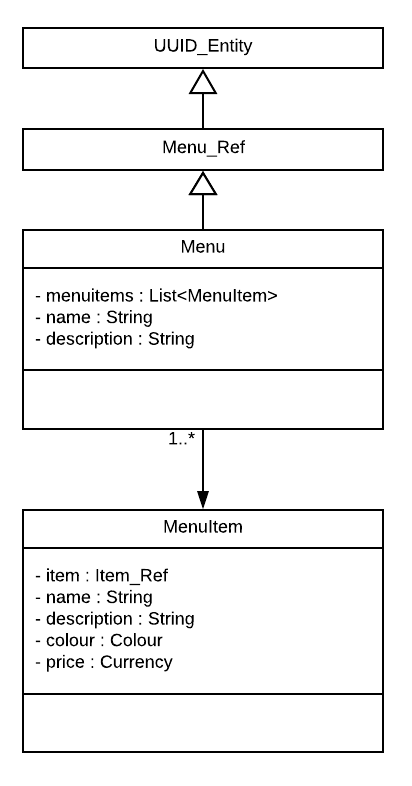
\includegraphics[width=\linewidth]{images/data_model/menu.png}
		\captionof{figure}{UML Menu Class}
	\end{minipage}

\pagebreak

\subsubsection{Item}
	\begin{figure}
		\centering
		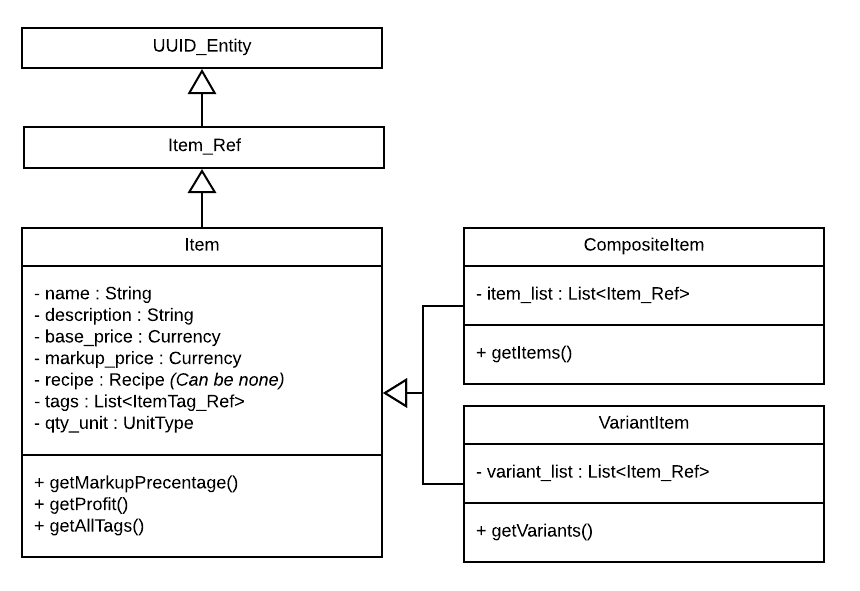
\includegraphics[width=.6\linewidth]{images/data_model/item.png}
		\caption{UML Item Class and Subclasses}
	\end{figure}

	Item class and its subclasses are used to model the process of ingredients inside a kitchen moving from storage into intermediary products and then finally finished products. It models this by using the Composite class pattern, where CompositeItem is the Composite class and Item is the leaf class. Using this pattern the system can represent heirarcys of ingredients into final products. For instance ground beef into patties and patties into burgers. This gives the user great flexibility and depth in representing production chains in the software and gives the software many metrics to provide functionality or statistics. The design deviates from the original gang of four's pattern by using an additional Composite class VariantItem. The purpose of variant item is to group similar items that can be interchanged in recipes. For instance gluten free bread and regular bread would be grouped in the variant item Bread. This allows for the system to dynamically adjust recipes by knowing which ingredients can be substituted to create different properties in the final product. Such as selecting that the final product be made from only gluten free ingredients. These features are only possible by having a seperate item model from menu items.
	
	The design was picked for robustness as the model makes no assumptions directly about selling food and can be fitted for any goods the user may want to sell. Since ingredients and products are the assumed to be the same in our system the user has complete control to ignore this feature if they wish to not engage with it and only list final products. They sacrifice features like order customisation, variants and percision stock control, but this is still supported to engage with the widest audience of stakeholders.
	
	An item consists of a base price and markup price. This is the price the user can buy the item for and the price the user sells the item for. The base price is used to calculate profit margins for the user and the markup price is used as the default sell price of menu item. This field is useful even for ingredients that will never be on a menu as it is used to calculate add on cost for order customisation discussed further in Section \ref{subsubsec:Order}.
	
	The qty unit on item is an enum to designate the quantity unit for stock. This could be kilogram, litre or count.
	

\subsubsection{ItemTag}

	\begin{minipage}[t]{.6\linewidth}
		ItemTag class can be created and applied by the user to designate collections of items under a similar tag, such as gluten free or vegan. The class has two attributes name and dominant flag. The dominant flag is used in descision making in the software to how the tag interacts in composite items. If a tag is dominant then the parent item inheirts the tag if it has one child that owns it. For instance 'Contains peanuts' would be considered a dominant tag because anything made using that tag would also contain peanuts. If a tag is non-dominant then the parent tag only inherits the tag if all its children have the tag. For instance 'gluten-free' is only true if all ingredients are also gluten free. 
		
	\end{minipage}
	\hspace{0.02\linewidth}
	\begin{minipage}[t][][b]{.3\linewidth}
		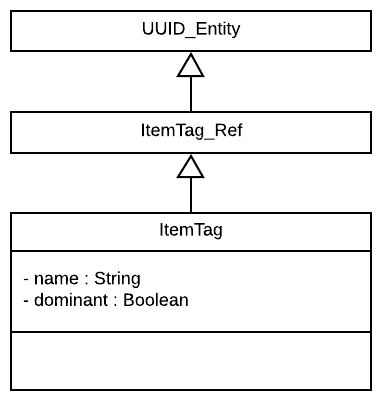
\includegraphics[width=\linewidth]{images/data_model/tag.png}
		\captionof{figure}{UML ItemTag Class}
	\end{minipage}


\subsubsection{StockInstance}
	\begin{minipage}[t]{.6\linewidth}
		The StockInstance class represents physical stock of an item that the user has. Using this information the system calculates what products can be made from the ingredients avaliable and warns when running low or close to expiry. The model uses a seperate stock instance class rather than a quantity attribute for item to better emulate the real world. From stakeholder surveys(Section \ref{Surveys}) managing inventory is an important feature and the pattern in which stakeholders bought ingredients was in discrete bulk lots with individual expiry dates. The stock instance class aims to models these bulk lots and give more detail to the system of  ingredients freshness and quantities.
		
	\end{minipage}
	\hspace{0.02\linewidth}
	\begin{minipage}[t][][b]{.3\linewidth}
		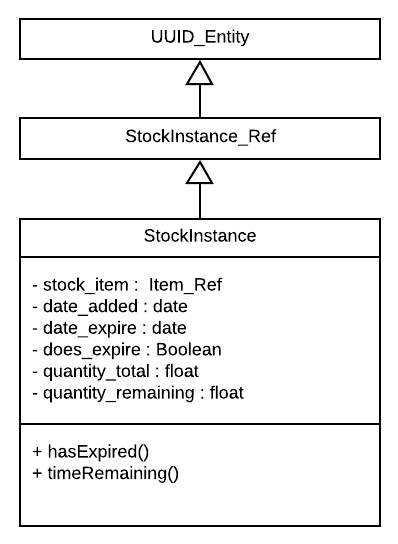
\includegraphics[width=\linewidth]{images/data_model/stock.png}
		\captionof{figure}{UML StockInstance Class}
	\end{minipage}

\subsubsection{Order} \label{subsubsec:Order}

	\begin{minipage}[t]{.6\linewidth}
		The Order class models an order made to the system for a single or multiple menu items. The order class was designed with the ability to customise the ingredients in the order by adding, replacing or removing. To accomplish this the Order has to be expressed in the same form as the items and so a heirarcy of OrderItems is used. This is created by deep copying Composite Items into OrderItems. For variant items the variantItem is added to the order and the first variant is added as its child. This is done to perserve the information of the variant item so it can be swaped for other variants. See Appendix \ref{Appendix orders} for an example of this conversion.
	\end{minipage}
	\hspace{0.02\linewidth}
	\begin{minipage}[t][][b]{.3\linewidth}
		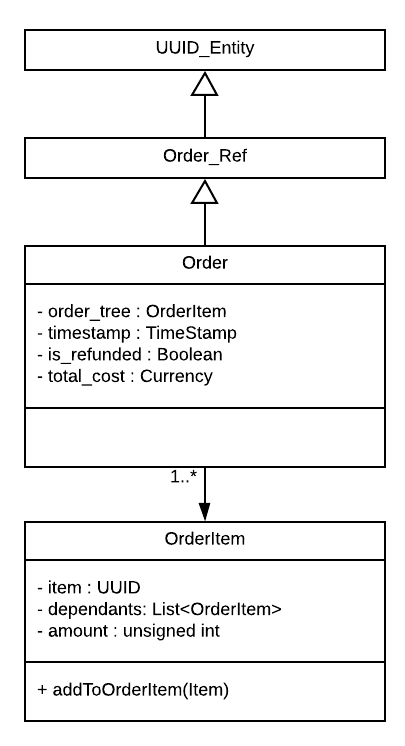
\includegraphics[width=\linewidth]{images/data_model/order.png}
		\captionof{figure}{UML Order Class}
	\end{minipage}

\pagebreak

\subsection{Architecture} \label{subsec:Architecture}
	\subsubsection{Model-View-Controller}
		The system was decided to use the Model View Controller design pattern for its architecture for the advantages of its low coupling of system and gui logic. The core of the data model is described with detail in Section \ref{subsec:DataModel}. To assist in the design of maintainable code the Controller was split into three sublayers of classes. Firstly Managers are identified systems of related code in the program that have shared state. They act as a linker foremost managing the access and use of shared state. The program has very litte state other than data model and so the only manager is OrderManager; That faciliates the order cart and the constuction and customisation of Orders.
		 Second is Logical Services that provide some single responsibility service to the higher levels of the program. An example of this in the software is DataQuery which provides a service of data filtering data model lists. 
		Lastly is GUI Controllers, which are in charge of data sanatation for lower layers and building of dynamic gui elements.
		Having these sublayers allows for finer control of single responsibility and low coupling. In turn making code more maintainable and easier to test. Below is a visual diagram of these layers.

		\begin{figure}[h]
			\centering
			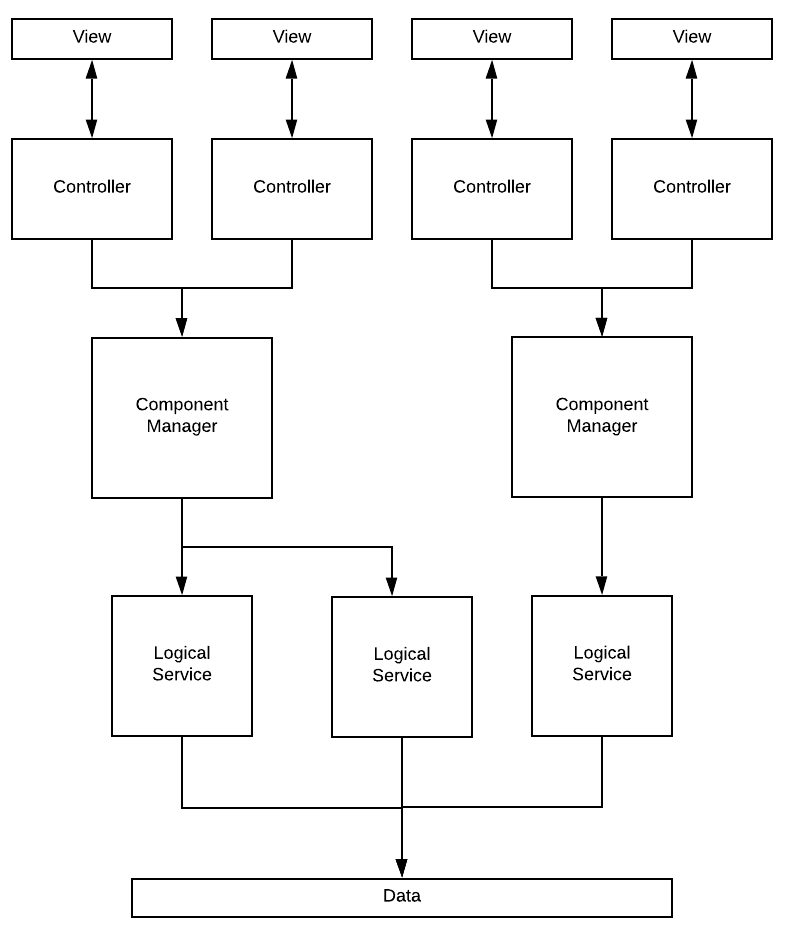
\includegraphics[width=.6\linewidth]{images/data_model/architecture.png}
			\caption{Software Layer Communication Diagram}
		\end{figure}

\pagebreak

\subsubsection{Data Persistence}
Data persistence was important to the project to give the user a Consistent(QR) view of the dataset in the application at all times. To ensure that data model changes were universal in the software the references to data model objects had to be the same through out the program. This was accomplished using a centralised storage system called StorageAccess. 

\begin{figure}[h]
	\centering
	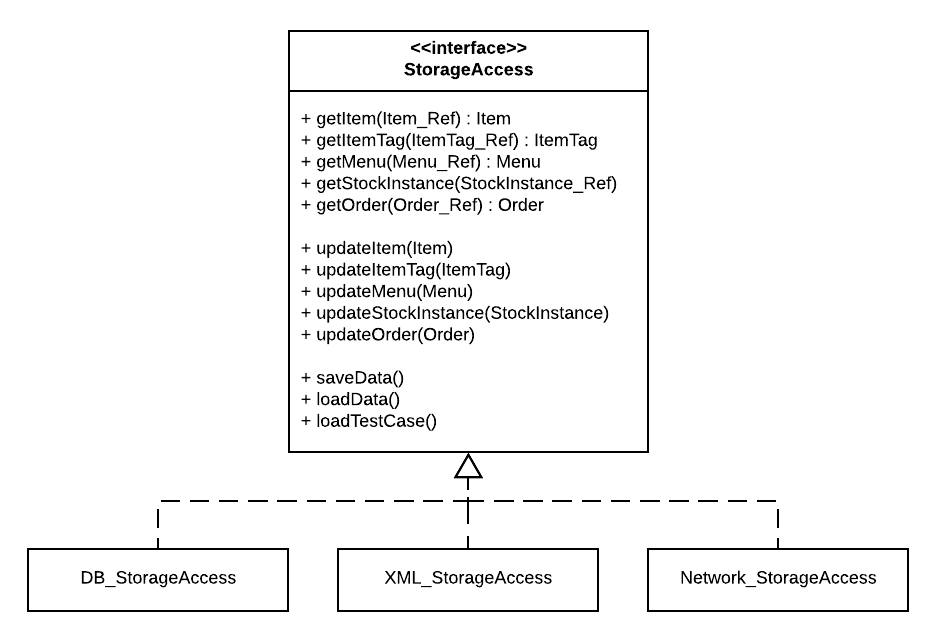
\includegraphics[width=.75\linewidth]{images/data_model/storage.png}
	\caption{UML StorageAccess Class Diagram}
\end{figure}

StorageAccess is an interface whos single responsibility is to convert data model objects from physical storage to the class objects. This interface is implemented by classes that provide a type of physical storage, for instance XML StorageAccess which saves and loads xml files into memory. This single interface allows for Flexibility(QR) in storage medium and means the program is open to upgradeability by changing the StorageAccess implementation. Storage access is a singleton since there is only need for one dataset loaded at a time in the system. The reason a single point of access for the dataset of the application is to increase maintainability in the code as it provides a single location to modify how data is stored or how the system reacts to updates. For example StorageAccess can implement the observable pattern and alert gui systems when it needs reload elements because of data updates. This sort of feature is much harder to maintain when you have multiple managers who keep track of this data, as you require multiple locations for the same logic. This creates stronger integration testing as you can better guarantee what data is loaded in the system via test data sets.

StorageAccess has get and update functions for all objects which need to be persistent between runs of the application. These persistent objects are refered to in Section \ref{subsec:DataModel}. 

To ensure that every persistent object has a primary key, A required attribute for many storage mediums, all persistent objects inherit from the UUID Entity class which randomly assigns a unique 128 bit number to that object. It also provides methods for comparing equality of two objects. UUID Entity is all that is needed to reference a persistent object, however StorageAccess and most classes use an object reference instead. Object References inherit from UUID Entity and have no additional attributes. They are used to provide an alias to UUID Entity and add context to code for what type of object the reference represents.

\pagebreak

\subsection{Design Post-Mortem} \label{subsec:TechnicalDesignPost}
\subsubsection{Investing in Architecture}
From reflection the hypothesis that investing in architecture would save developer time and create more maintainable(QR) and flexible(QR) was correct. Most systems are well isolated and only communicate with services that it uses(reduced coupling). There is no god classes in the application and a large majority of classes have strict single responsibility. This has allowed the code to be very easily extendable. An example of this is the feature of auto-saving. By having StorageAccess solely responsible for persistence of data adding auto saving was trivial by calling save data method on any modification to the persistent state, effectively introducing auto save on any committed changes. This is a single example however the time savings are more revealed in the absence of infrastructure road blocks. Not once in the project was there a feature which was incompatible with the design of the system requiring work around solutions, everything had a place. This is a hard claim to proof so we can only refer to the commit logs as proof of this.

\subsubsection{Design Reflections}
XML was chosen as the default to meet client requirements for import and export of XML data and while useful is not suited for being the primary StorageAccess implementation used.
XML is designed to be human readable and editable however this comes at the cost of processing speed and storage. This trade off is not worth it in the current implementation
as it is not expected that most users are manually editing the file but modifying data through the use of the application. It therefore makes sense to refactor this system into a more binary format
to speed up the program and reduce data size. If given more time this would be a futher step.\\

Autosaving as it stands works well, due to the issues mentioned above however autosaving will cause stutters as the application grows due to the requirements of JAXB(XML Library) to save the whole file on change.
There are several mitagating factors that could be implemented to accomadate for this while still using XMl; These are mentioned in XML Storage Class header in the code base. \\